\chapter{Properties}
\paragraph{} After five days of running from the goose police, Duckie was certain that he had escaped. He decided to stop and eat dinner, but just as he began to land, \textbf{Squawk!} He ran headfirst into another goose. 
\paragraph{} "Hold it right there! You need to come back with me to the village!" the policegoose demanded, slightly dazed. 
\paragraph{} "It's dangerous in the outside world. This is for your own safety!"
\paragraph{} Duckie knew that the policegoose, named Güs was rational and decided to try to reason with him. "Of course it's dangerous! But I have to do this. I am looking for the golden goose of legend. The one who is supposed to save us, change all of goose society and help us through our migrations."
\paragraph{} "But that's against the rules! Why would you risk your life to break their rules? Don't they keep us safe?" Güs asked.
\paragraph{} "Its true. Some of the rules do keep us same, but too many take away our liberty. I think they are afraid of what will happen if I find the golden goose. If I can find her, then they may not be able to stay in power. You joined the goose police to help people, and if you let me go, you can do just that!"
\paragraph{} "You might be right, but I can't betray the village. If I just let you go without at least trying to stop you, I won't be able to look myself in the mirror, much less be seen in the village! I have no interest in fighting, so I'll tell you what. I will have a set of challenges with you. If you beat me, I will let you go. If not, you have to let me take you back. Sound fair?"
\paragraph{} Duckie was reluctant, but knew that he had no other options. "Fine. Let's do the challenges."
\pagebreak
\subchapter{Associativity}
{Güs and Duckie both felt that they were good fliers. 
\paragraph{} "To begin, let's do a flying contest in 3 parts." Gus announced. "Whoever flies the furthest wins."
\paragraph{} Duckie thought about this. "Fine, but to make sure no one gets an unfair advantage, let's allow one break in between."
\paragraph{} The first leg of the race was $1 km$, the second leg was $\mathbf{2} km$, and the third leg was $\mathbf{1} km$. Duckie and Güs both wanted to win, so created strategies. Güs decided to travel the first leg ($\mathbf{1} km$) of the race, took his break then travel the second and third legs ($\mathbf{2} km$ and $\mathbf{1} km$). Duckie instead traveled the first leg, ($\mathbf{1} km$) of the race and the second leg ($\mathbf{2} km$) of the race, then took his break, and traveled the third leg ($\mathbf{1} km$). Did they tie by traveling the same amount?}
{Yes! Duckie traveled $(\mathbf{1} km + \mathbf{2} km) + \mathbf{3} km = \mathbf{5} km$. Güs traveled $\mathbf{1} km + (\mathbf{2} km + \mathbf{3} km) = \mathbf{5}km$. Duckie and Güs both traveled $\mathbf{5km}$.}
{Adding can be grouped in any way. In other words: (A+B)+C = A+(B+C).}
{\begin{tikzpicture}
    \coordinate (A) at (0,0);
    \coordinate (B) at (0,2);
    \coordinate (C) at (0,6);
    \coordinate (D) at (0,8);
    \coordinate (Ap) at (1.5,0);
    \coordinate (Bp) at (1.5,2);
    \coordinate (Cp) at (1.5,6);
    \coordinate (Dp) at (1.5,8);

    \node [inner sep=0pt] at (D) {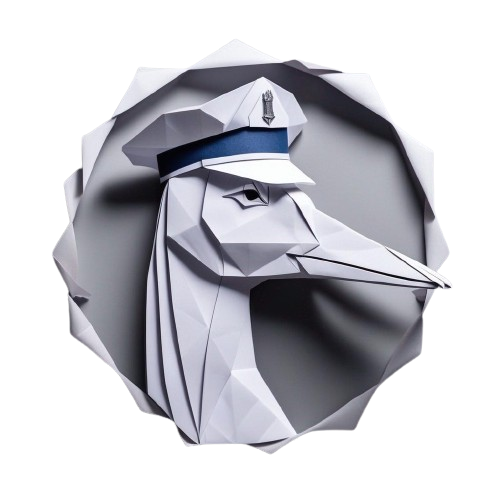
\includegraphics[height=0.8cm]{Gus}};
    \draw[-|,ultra thick,red, decorate, decoration={random steps,segment length=3pt,amplitude=0.2pt}] (A) -- (B) node[midway, left] {$1 km$};
    \draw[->,ultra thick,blue, decorate, decoration={random steps,segment length=3pt,amplitude=0.2pt}] (B) -- (C) node[midway, left] {$2 km$};
    \draw[->,ultra thick,violet, decorate, decoration={random steps,segment length=3pt,amplitude=0.2pt}] (C) -- (D) node[midway, left] {$1 km$};

    \node [inner sep=0pt] at (Dp) {
\includegraphics[height=0.8cm]{DuckieGami}};
    \draw[->,ultra thick,red, decorate, decoration={random steps,segment length=3pt,amplitude=0.2pt}] (Ap) -- (Bp) node[midway, left] {$1 km$};
    \draw[-|,ultra thick,blue, decorate, decoration={random steps,segment length=3pt,amplitude=0.2pt}] (Bp) -- (Cp) node[midway, left] {$2 km$};
    \draw[->,ultra thick,violet, decorate, decoration={random steps,segment length=3pt,amplitude=0.2pt}] (Cp) -- (Dp) node[midway, left] {$1 km$};

    \draw [decorate,
	decoration = {brace,mirror,
		raise=15pt,}] (Ap) -- (Dp) node[midway, right, xshift=0.8cm] {$4 km$};
\end{tikzpicture}
}
%Additive Commutativity
\subchapter{Additive Commutativity}
{Duckie and Güs sat down, tired. They had each expected to win, and had surprised each other. 
\paragraph{} "What should we do? Will you let me go?" Duckie asked hopefully. \paragraph{} Güs thought about this. "No, but I will let you try to beat me again" 
\paragraph{} Because geese are water animals, swimming is a very important skill, so they decided to swim for their next competition. They each had a different strategy. Güs swam $\mathbf{140} m$, dried off, then swam $\mathbf{160} m$. Duckie instead swam $\mathbf{160} m$, dried off, then swam $\mathbf{140} m$. Did they tie?}
{Yes! Güs flew $\mathbf{140} m + \mathbf{160} m = \mathbf{300} m$. Duckie instead flew $\mathbf{160} m + \mathbf{140} m = \mathbf{300} m$. They swam the same amount.}
{Order doesn't matter when adding. In other words: A+B = B+A.}
{\begin{tikzpicture}
    \coordinate (A) at (0,0);
    \coordinate (B) at (0,4);
    \coordinate (C) at (0,9);
    \coordinate (Ap) at (1.5,0);
    \coordinate (Bp) at (1.5,5);
    \coordinate (Cp) at (1.5,9);
    
    \node [inner sep=0pt] at (C) {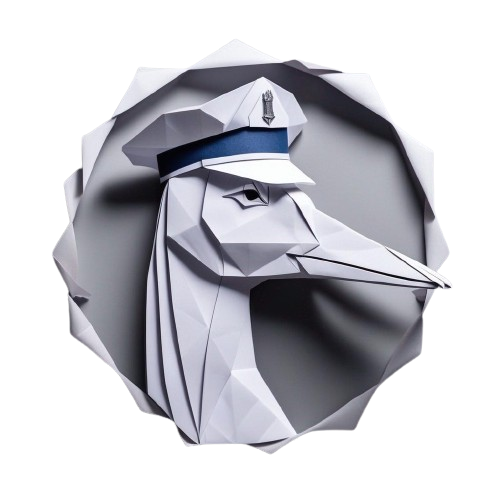
\includegraphics[height=0.8cm]{Gus}};
    \draw[->,ultra thick,red, decorate, decoration={random steps,segment length=3pt,amplitude=0.2pt}] (A) -- (B) node[midway, left] {$\distanceTwoTwoO m$};
    \draw[->,ultra thick,blue, decorate, decoration={random steps,segment length=3pt,amplitude=0.2pt}] (B) -- (C) node[midway, left] {$\distanceTwoTwoTw m$};
    
    \node [inner sep=0pt] at (Cp) {
\includegraphics[height=0.8cm]{DuckieGami}};
    \draw[->,ultra thick,blue, decorate, decoration={random steps,segment length=3pt,amplitude=0.2pt}] (Ap) -- (Bp) node[midway, left] {$\distanceTwoTwoTw m$};
    \draw[->,ultra thick,red, decorate, decoration={random steps,segment length=3pt,amplitude=0.2pt}] (Bp) -- (Cp) node[midway, left] {$\distanceTwoTwoO m$};
    
    \draw [decorate, 
	decoration = {calligraphic brace,mirror,
		raise=10pt,amplitude=5pt}] (Ap) -- (Cp) node[midway, right, xshift=0.5cm,line width=3pt] {$\distanceTwoTwoF m$};
\end{tikzpicture}}
%Distributivity
\subchapter{Distributivity}
{Duckie and Güs were starting to get frustrated. 
\paragraph{} "How are we going to get around this?" Güs asked.
\paragraph{} Duckie thought for a moment. He knew Güs could only compete for so long before becoming tired, and the more they flew, the better chance he would have. "How about a flying contest? We can do four parts instead of just three. Maybe then one of us will win."
\paragraph{} Gus agreed. His training from the goosepolice had given him excellent stamina, and was confident he could beat Duckie in long distance flying. 
\paragraph{} In the third contest, Güs traveled $\mathbf{2} km$, then $\mathbf{3} km$, and repeated that pattern $\mathbf{2}$ times. Duckie instead traveled $\mathbf{2} km$ $\mathbf{2}$ times, then $\mathbf{3} km$ $\mathbf{2}$ times. Did they tie?}
{Yes! Duckie flew $\mathbf{2}\ast(\mathbf{2} km + \mathbf{3} km)$, or $\mathbf{10} km$, and Güs flew $\mathbf{2}\ast\mathbf{2} km \ast \mathbf{3}\ast\mathbf{2} km$, or $\mathbf{10}km$.}
{Multiplying with an expression is the same as multiplying with each part of the expression. In other words: A$\ast$(B+C) = (A$\ast$B) + (A$\ast$C).}
{}
%Commutativity
\subchapter{Multiplicative Commutativity}
{At this point, Güs realized that Duckie was a very capable goose. When he first challenged Duckie, he expected winning to be a cakewalk, but Duckie ended up posing quite a challenge. Seeing Duckie's perseverance, Güs began to respect Duckie. He decided to give him another chance. He decided that the next contest should be a weightlifting competition, where whoever lifted the most amount of total weight would win. Duckie lifted $\mathbf{10} kg$  $\mathbf{3}$ times, whereas Güs lifted only $\mathbf{3} kg$ but did it $\mathbf{10}$ times. Did they tie?}
{Yes! Duckie lifted $\mathbf{10}kg\ast\mathbf{3}=\mathbf{30}kg$, and Duckie lifted $\mathbf{3}kg \ast \mathbf{10}=\mathbf{30}kg$. They lifted the same amount.}
{When multiplying, order does not matter. In other words: A$\ast$B = B$\ast$A.}
{\begin{tikzpicture} 
    \node [inner sep=0pt] at (0,15) {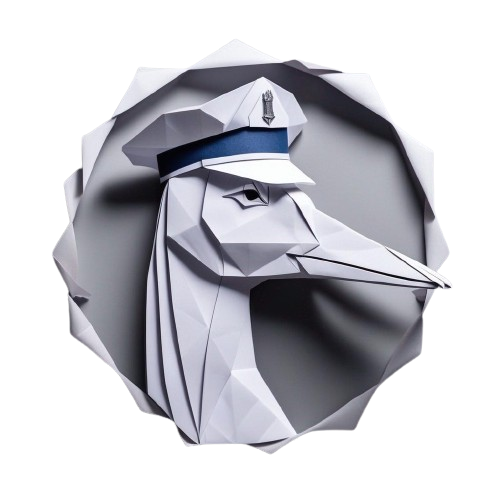
\includegraphics[height=0.8cm]{Gus}};
    \foreach \pos in {1,...,10} {	
        \MODULO{\pos}{2}{\rval}
        \SUBTRACT{\pos}{1}{\bl}
        \MODULO{\bl}{2}{\bval}
        \definecolor{col}{rgb}{\rval,0,\bval}
        \draw[->,ultra thick,col, decorate, decoration={random steps,segment length=3pt,amplitude=0.2pt}] (0,\pos *1.5 - 1.5) -- (0,\pos *1.5) node[midway, left] {$3 kg$};
    }
     \node [inner sep=0pt] at (1.5,15) {
\includegraphics[height=0.8cm]{DuckieGami}};
    \foreach \pos in {1,...,3} {	
        \MODULO{\pos}{2}{\rval}
        \SUBTRACT{\pos}{1}{\bl}
        \MODULO{\bl}{2}{\bval}
        \definecolor{col}{rgb}{\rval,0.7,\bval}
        \draw[->,ultra thick,col, decorate, decoration={random steps,segment length=3pt,amplitude=0.2pt}] (1.5,\pos *5 - 5) -- (1.5,\pos *5) node[midway, left] {$10 kg$};
    }
    
    \draw [decorate, decoration = {calligraphic brace,mirror, raise=10pt,amplitude=5pt}] (1.5,0) -- (1.5,15) node[midway, right, xshift=0.5cm,line width=3pt] {$30 kg$};
\end{tikzpicture}}
\paragraph{} Duckie and Güs landed on the forest floor, exhausted. They had realized that, no matter what the competition was, they were equally matched. They hadn't beat each other, but they \textit{had} won each other's respect. 
\paragraph{} "Why don't you join me?. You can make a difference!" asked Duckie.
\paragraph{} "I can't!" Güs cried. "What about my life in the goose police?"
\paragraph{} "Well, do you believe the golden goose is out there?"
\paragraph{} "Honestly, I'm not sure. Do you really think it will make the village a better place?"
\paragraph{} Duckie knew that there was the possibility the golden goose was a hoax, but knew the danger of disobeying the goose authorities, but knew he could help the entire village. 
\paragraph{} "You joined the goose police to help people", he reasoned. "You are clearly capable of making the dangerous journey, and if you can join me, you can do exactly that."
\paragraph{} Güs knew he was right. While he was afraid of what could happen along the journey, deep down, knew the tyranny of the authorities had gone too far. He decided to be brave and join Duckie. 
\paragraph{} "All right. I will join you!" he said resolutely. 